\subsection{Passer le péage}
\subsubsection{Scénario Cockburn}
\textbf{Cas d'utilisation:} Passer le péage
    
\textbf{Acteur primaire (initiateur):} Le conducteur
    
\textbf{Pré-condition: } Nécessite que la voie soit ouverte et libre.
    
\textbf{Post-condition: }   La voie redevient disponible(ouverte et libre) pour un prochain usager.
    
\textbf{Scénario primaire: } \\
\textbf{1.} Le conducteur rentre dans la voie d’autoroute.%(\ref{subsec:rentre})
 \\
\textbf{2.} Le conducteur paye le passage. %(\ref{subsec:paie})
\\
\textbf{3.} Le conducteur sort. %(\ref{subsec:sortir})
\\
    
\textbf{Variantes}\\
\textbf{1a.}  Le conducteur n’arrive pas a rentrer dans la voie, il appelle le technicien et fin du scénario.\\
\newpage
\subsubsection{\textbf{Décomposition des cas d'utilisation:}}
\begin{figure}[h]
    \centering
    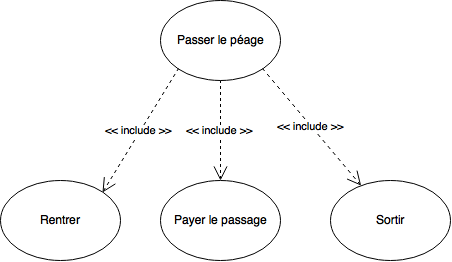
\includegraphics[scale=0.5]{02_Desenvolvimento/TD2/images/PasserLePeage.png}
    \caption{Décomposition de cas d'utilisation: Passer le péage}
\end{figure}
\newpage
\subsubsection{\textbf{Diagramme de activité:}}
\begin{figure}[h]
    \centering
    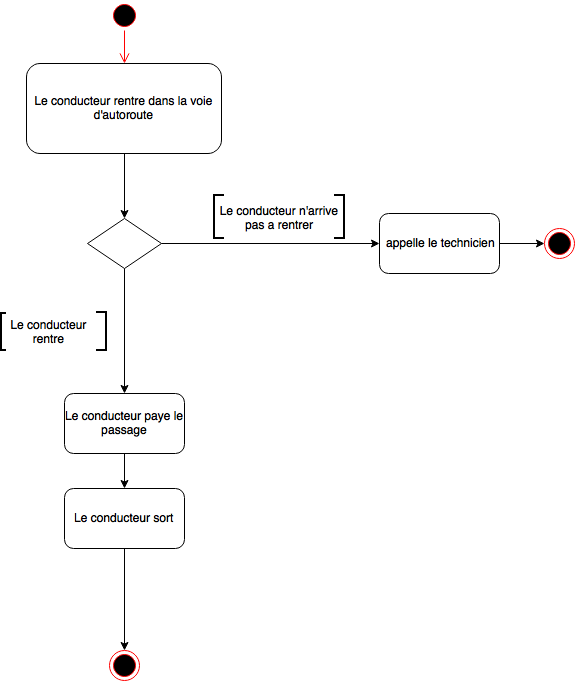
\includegraphics[scale=0.6]{02_Desenvolvimento/TD2/images/DAPasserPeage.png}
    \caption{Décomposition de cas d'utilisation: Passer le péage}
\end{figure}